\documentclass[a4paper]{article}
\usepackage[landscape]{geometry}
\usepackage{url}
\usepackage{multicol}
\usepackage{amsmath}
\usepackage{esint}
\usepackage{amsfonts}
\usepackage{tikz}
\usetikzlibrary{decorations.pathmorphing}
\usepackage{amsmath,amssymb}

\usepackage{colortbl}
\usepackage{xcolor}
\usepackage{mathtools}
\usepackage{amsmath,amssymb}
\usepackage{enumitem}
\usepackage[pdftex]{graphicx}
\makeatletter

\newenvironment{tablehere}
  {\def\@captype{table}}
  {}

\newenvironment{figurehere}
  {\def\@captype{figure}}
  {}

\newcommand*\bigcdot{\mathpalette\bigcdot@{.5}}
\newcommand*\bigcdot@[2]{\mathbin{\vcenter{\hbox{\scalebox{#2}{$\m@th#1\bullet$}}}}}
\makeatother

\title{RoVi CheatSheet}
\usepackage[brazilian]{babel}
\usepackage[utf8]{inputenc}

\advance\topmargin-.8in
\advance\textheight3in
\advance\textwidth3in
\advance\oddsidemargin-1.5in
\advance\evensidemargin-1.5in
\parindent0pt
\parskip2pt
\newcommand{\hr}{\centerline{\rule{3.5in}{1pt}}}
%\colorbox[HTML]{e4e4e4}{\makebox[\textwidth-2\fboxsep][l]{texto}
\begin{document}

\begin{center}{{\textbf{RoVi Cheat Sheet (Robotics)}}}\\
\end{center}
\begin{multicols*}{3}

\tikzstyle{mybox} = [draw=black, fill=white, very thick,
    rectangle, rounded corners, inner sep=10pt, inner ysep=10pt]
\tikzstyle{fancytitle} =[fill=black, text=white, font=\bfseries]

%------------ Note ---------------
\begin{tikzpicture}
\node [mybox] (box){%
    \begin{minipage}{0.3\textwidth}
        Euler Angles Fixed: XYZ - $(\psi, \Theta, \phi)$, Movable: ZYX$(\alpha, \beta, \gamma)$)
        \\
        \textbf{Quaternions:} 
        \begin{align*}
            q &= [w, \textbf{v}]\\
              &= [w, x\textbf{i} + y \textbf{j}, z \textbf{k}]\\
              &= w, x\textbf{i} + y \textbf{j}, z \textbf{k}
        \end{align*}
        $q_a, q_b$ \\
        Addition:
        $[w_a + w_b, (x_a+x_b) \textbf{i} (y_a+y_b) \textbf{j} (z_a+z_b) \textbf{k}]$ \\
        Mult: 
        $ [w_a w_b - \textbf{v}_a \cdot \textbf{v}_b, w_a \textbf{v}_b + w_b \textbf{v}_a + \textbf{v}_a \times \textbf{v}_b  ]$        \textbf{Non-comm} 
        Conjucation: $ [w, \textbf{v} ] \rightarrow [w, \textbf{-v} ] $, $qq^* = |q|^2$ (norm$^2$) \\
        Inverse: $ q^{-1} = \frac{q^*}{|q|^2}$ Inverse of unit quat is conjucated 
    \end{minipage}
};
%------------ Header ---------------------
\node[fancytitle, right=10pt] at (box.north west) {Rotations};
\end{tikzpicture}

\begin{tikzpicture}
\node [mybox] (box){%
    \begin{minipage}{0.3\textwidth}
        \begin{figurehere}
            \centering
            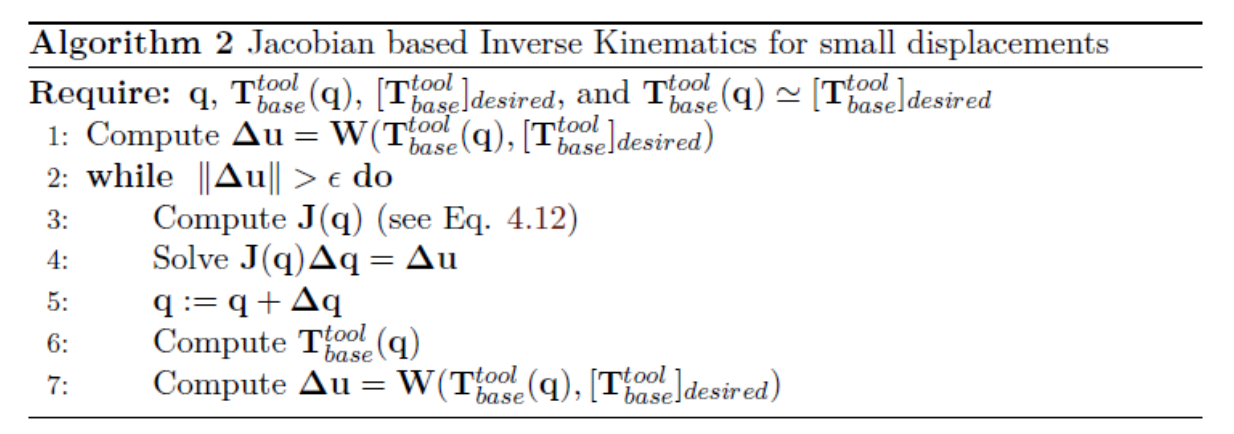
\includegraphics[width=1\textwidth]{images/alg_2.png}
        \end{figurehere}
    \end{minipage}
};
%------------ Header ---------------------
\node[fancytitle, right=10pt] at (box.north west) {Inverse Kinematics};
\end{tikzpicture}

\begin{tikzpicture}
\node [mybox] (box){%
    \begin{minipage}{0.3\textwidth}
        Interpolation: \\
        $q_t = \frac{\sin(1-t)\theta}{\sin(\theta)} q_1 + \frac{\sin(t\theta)}{\sin(\theta)}q_2$\\
        Angle between Quaternions: \\
        $ \cos{\theta} = \frac{q_1 \cdot q_2}{|q_1||q_2|} = \frac{ w_1w_2+x_1x_2+y_1y_2+z_1z_2 }{ |q_1||q_2| } $\\
        $ \theta = \cos^{-1}\left({\frac{ w_1w_2+x_1x_2+y_1y_2+z_1z_2 }{ |q_1||q_2| }\right) $ Note: Maybe half angle (*2)

        If the dot product is negative, the long way is chosen, negate one q to get shortest.

        \textbf{MATLAB:} 
        SLERP: \texttt{$q_0$ = slerp($q_1$,$q_2$,1/100)} \\
        quat as vector: \texttt{q.compact}
        


    \end{minipage}
};
%------------ Header ---------------------
\node[fancytitle, right=10pt] at (box.north west) {Quaternion interpolation};
\end{tikzpicture}

\begin{tikzpicture}
\node [mybox] (box){%
    \begin{minipage}{0.3\textwidth}
        
        \begin{figurehere}
            \centering
            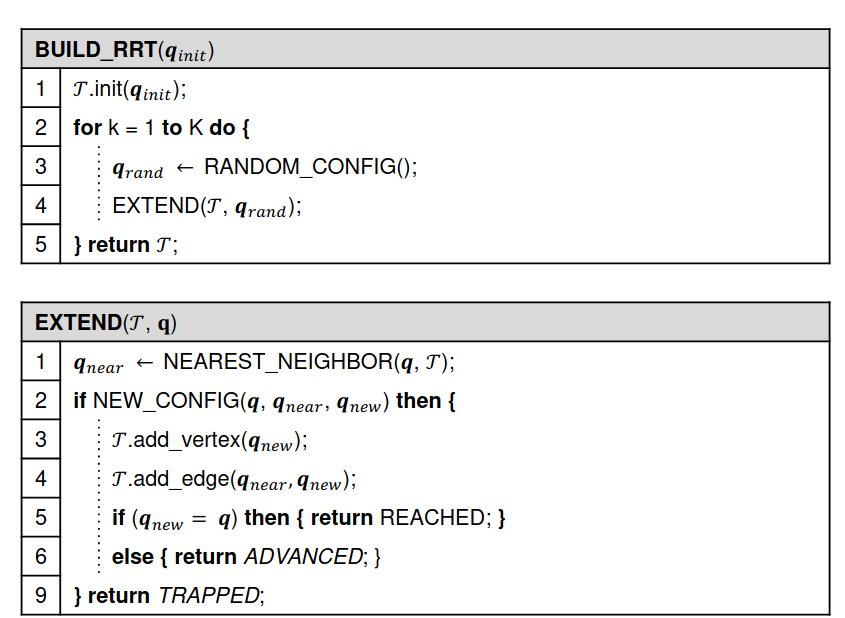
\includegraphics[width=0.8\textwidth]{images/rrt.png}
        \end{figurehere}
        \\
        
        \begin{figurehere}
            \centering
            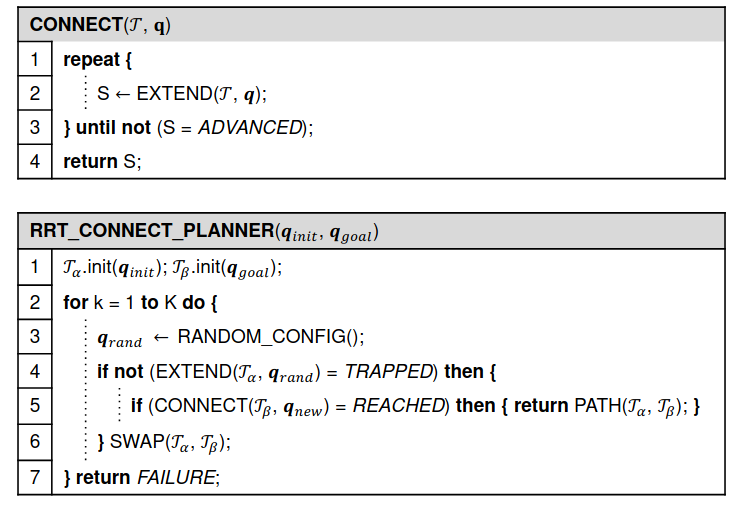
\includegraphics[width=0.8\textwidth]{images/rrtconnect.png}
        \end{figurehere}
    \end{minipage}
};
%------------ Header ---------------------
\node[fancytitle, right=10pt] at (box.north west) {RRT};
\end{tikzpicture}

\begin{tikzpicture}
\node [mybox] (box){%
    \begin{minipage}{0.3\textwidth}
        
        Positional: $ q_{min} \leq q + \Delta q \leq q_{max}  $ \\
        Velocity: $ v_{min} \Delta t_i \leq \Delta q \leq v_{max}\Delta t_i $ , $ \Delta t_i = t_i+1-t_i $
        Velocity (add q): $ v_{min} \Delta t_i+q \leq q+\Delta q \leq v_{max}\Delta t_i+q $ 
        Acceleration: $ \Delta q = \frac{1}{2} a \Delta t_i [\Delta t_{i-1} + \Delta t_i] + \frac{\Deltat_i}{\Delta t_{i-1}} (q^i - q^{i-1}) $
        \begin{align*}
            Q_{min}(q^i.q^{i-1},t_i) &= max\{ q_{min}, v_{min}, \Delta t_i + q^i, \frac{1}{2} a_{min} \Delta t_i [\Delta t_{i-1} + \Delta t_i] + \frac{\Deltat_i}{\Delta t_{i-1}} (q^i - q^{i-1}) \} \\
            Q_{max}(q^i.q^{i-1},t_i) &= min\{ q_{max}, v_{max}, \Delta t_i + q^i, \frac{1}{2} a_{max} \Delta t_i [\Delta t_{i-1} + \Delta t_i] + \frac{\Deltat_i}{\Delta t_{i-1}} (q^i - q^{i-1}) \} \\
            Q_{min}(q^i.q^{i-1},t_i) &\leq q+\Delta q \leq Q_{max}(q^i.q^{i-1},t_i)
        \end{align*}
        
        
    \end{minipage}
};
%------------ Header ---------------------
\node[fancytitle, right=10pt] at (box.north west) {Joint Limits};
\end{tikzpicture}
\begin{tikzpicture}
\node [mybox] (box){%
    \begin{minipage}{0.3\textwidth}
        tst
    \end{minipage}
};
%------------ Header ---------------------
\node[fancytitle, right=10pt] at (box.north west) {Placeholder};
\end{tikzpicture}
\begin{tikzpicture}
\node [mybox] (box){%
    \begin{minipage}{0.3\textwidth}

        MATLAB: \texttt{Polyfit(X,Y,N)}: Fit a N degree Polynomial
        MATLAB: \texttt{polyval(p,x)}: Evaluate Polynomial on x
        SPLINE: \begin{verbatim}
tq = 0:0.1:5;
slope0 = 0;
slopeF = 0;
xq = spline(t,[slope0; x; slopeF],tq);
yq = spline(t,[slope0; y; slopeF],tq);
        \end{verbatim}

    \end{minipage}
};
%------------ Header ---------------------
\node[fancytitle, right=10pt] at (box.north west) {Polynomial Interpolation};
\end{tikzpicture}
\end{multicols*}

\newpage


\begin{center}{{\textbf{RoVi Cheat Sheet (Vision)}}}\\
\end{center}
\begin{multicols*}{3}

\tikzstyle{mybox} = [draw=black, fill=white, very thick,
    rectangle, rounded corners, inner sep=10pt, inner ysep=10pt]
\tikzstyle{fancytitle} =[fill=black, text=white, font=\bfseries]

%------------ Note ---------------
\begin{tikzpicture}
\node [mybox] (box){%
    \begin{minipage}{0.3\textwidth}
        \begin{itemize}
            \item Calibration
            \item epipole 
            \item Plucker linjer
            \item Fundamental matrix
        \end{itemize}
    \end{minipage}
};
%------------ Header ---------------------
\node[fancytitle, right=10pt] at (box.north west) {TODO};
\end{tikzpicture}

%------------ Note ---------------
\begin{tikzpicture}
\node [mybox] (box){%
    \begin{minipage}{0.3\textwidth}
        Point on line: dot product is zero
    \end{minipage}
};
%------------ Header ---------------------
\node[fancytitle, right=10pt] at (box.north west) {Projective space};
\end{tikzpicture}
\end{multicols*}

\end{document}
